\section{Introduction}

	\subsection{The Standard Model of Particle Physics}

    Central to the moden age of particle physics in the standard model,

    \begin{multline} \label{eqn:std-mod}
      L_{GWL} = \sum_{f} ( \bar{\Psi}_{f} ( i \gamma^\mu \partial \mu - m_{f} ) \Psi_{f} - eQ_{f} \bar{\Psi}_{f} \gamma^\mu \Psi_{f} A_{\mu} ) + \frac{g}{\sqrt{2}} \sum_{i} ( \bar{a}^i_L \gamma^\mu b^i_L W^+_\mu + \bar{b}^i_L \gamma^\mu a^i_L W^-_\mu )                        \\                           
              + \frac{g}{2x_w} \sum_f \bar{\Psi}_f \gamma^\mu ( I^3_f - 2s^2_w Q_f - I6e_f \gamma_5 ) \Psi_f Z_\mu - \frac{1}{4} | \partial_\mu A_v - \partial_v A_\mu - ie(W^-_\mu W^+_v - W^+_\mu W^-_v ) |^2                                         \\                                     
              - \frac{1}{2} | \partial_\mu W^+_v - \partial_v W^+_\mu - ie ( W^+_\mu A_v - W^+_v A_\mu ) + ig' c_w (W^+_\mu Z_v - W^+_v Z_\mu |^2 \\
              - \frac{1}{4} | \partial_\mu Z_v - \partial_v Z_\mu + ig' c_w (W^-_\mu W^+_v - W^+_\mu W^-_v ) |^2 - \frac{1}{2} M^2_\eta \eta^2  - \frac{gM^2_\eta}{8M_W} \eta^3  - \frac{g'^2 M^2_\eta}{32M_W}\eta^4    \\     
              + | M_W W^+_\mu + \frac{g}{2} \eta W^+_\mu |^2 + \frac{1}{2} | \partial_\mu \eta + i M_Z Z_\mu + \frac{ig}{2c_w} \eta Z_\mu |^2 - \sum_f \frac{g m_f}{2 M_W} \bar{\Psi}_f \Psi_f \eta.                                                                                
    \end{multline}

    The standard model, shown in equation \ref{eqn:std-mod}, is a quantum field theory that discribes the fundermental particles and how they interact.
    While this essay does require, or attempt, to understand the intricate detail of the stardard model;
    the aim of many particle physics experiments is to Test, measure and varify the model.
    Dispite being the current best theory to explain particle interactions, the model is not complete.
    There are many undescribed phemimina, such as the matter domination in the universe, that require physics behond the standard model.
    To that end, major international efforts, namely in the form of the Large Hardrom Collider, aim to further knowledge and understanding of the underlying physics of the universe. \cite{ref:std-mod}

  \subsection{The LHCb Experiment}

    One such Experiment and the Large Hadrom Colider is Large Hadron Colider beauty (LHCb).
    Located at intersection point 

    \begin{figure}[ht]
      \centering
      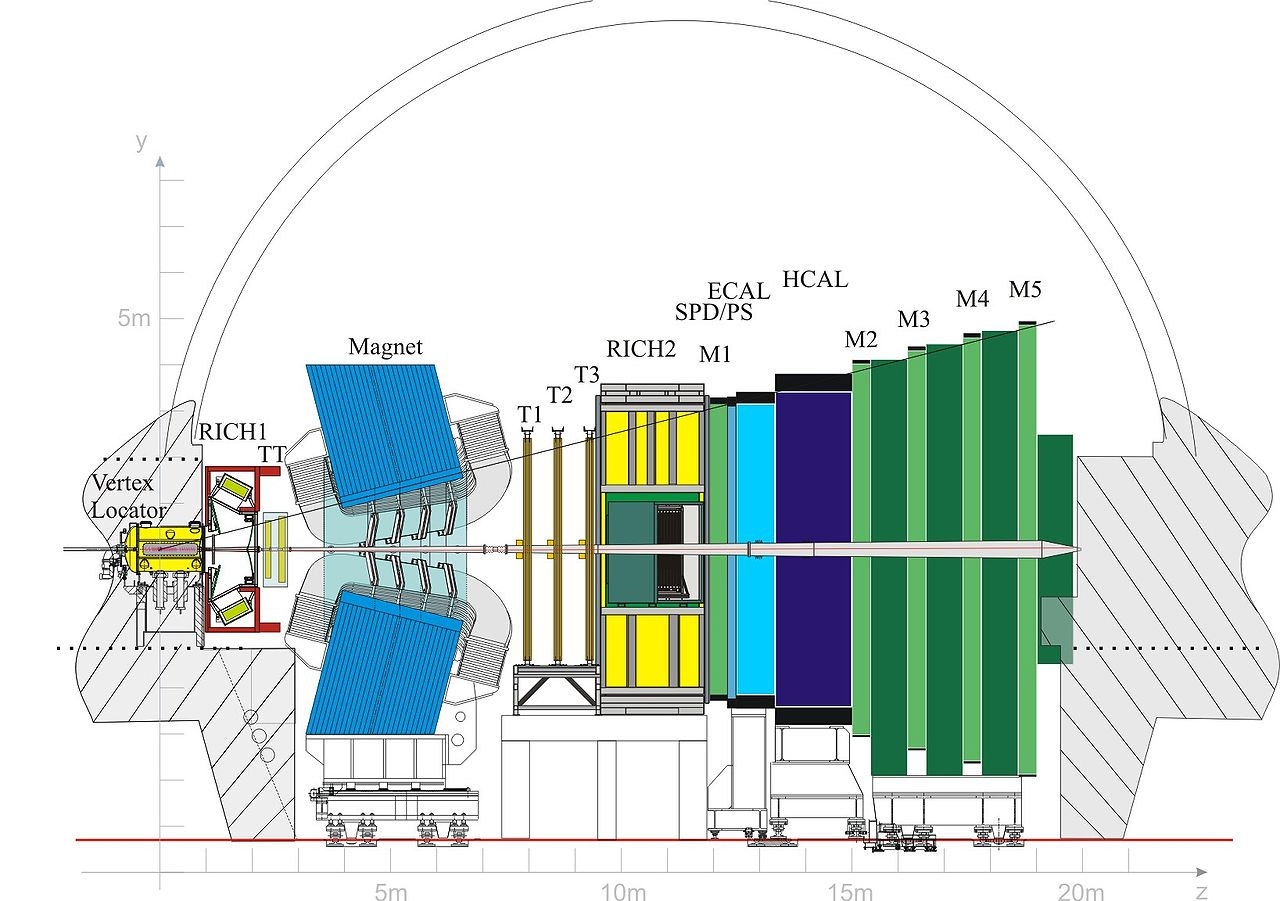
\includegraphics[scale=0.5]{LHCb_Det.jpg}
      \caption{The LHCb Detector along the bending plane.}
      \label{fig:LHCb_Collab}
    \end{figure}


  \subsubsection{The Detector}

  \subsubsection{Physics Studied at LHCb}

  \subsubsection{VELO Upgrade}

  \subsection{FPGAs in Particle Detectors}

  \subsubsection{Field Programable Gate Arrays}

  \subsubsection{The Role of FPGA's in the VELO Upgrade}
